\documentclass[12pt]{article}

\usepackage{sbc-template}
\usepackage[utf8]{inputenc}
\usepackage[brazil]{babel}
\usepackage{graphicx}
%\usepackage{booktabs}
\usepackage{amsmath}
\usepackage{hyperref}


\title{Visualização de Dados -- Trabalho Prático 1}

\author{Danilo Ferreira, Guilherme Avelino, Hudson Borges, Mauri Miguel}


\address{Departamento de Ciência da Computação, UFMG
%\email{\footnotesize \{danilofs,mtov\}@dcc.ufmg.br}
}


\begin{document}

\maketitle

%\section{Introdução}
\begin{abstract}
Neste trabalho desenvolvemos uma visualização que representa uma série de comunidades de pessoas que visitam diferentes lugares. O principal objetivo da visualização é identificar os padrões de locais visitados e semelhanças entre as pessoas e comunidades.\\
\centerline{\url{http://dcc.ufmg.br/~danilofs/dvis/tp1}}
\end{abstract}


\section{Abordagem Proposta}

O trabalho tem por objetivo a análise visual de um conjunto de grafos bipartidos e identificar semelhanças entre eles. Nessa abordagem trabalhamos a visualização dos dados de forma que facilite a identificação de nós semelhantes no grafo, distinguindo os nós que possuem um nó semelhante em todos os grafos dos que não possuem. Mais especificamente, a visualização possui as seguintes características:
\begin{itemize} 
	\item Cada grafo é apresentado separadamente em um gráfico, sendo a seleção do grafo a ser visualizada disponibilizada através de uma aba lateral.
	\item Cada nó é representada por um círculo multicolorido (\textit{donuts}). 
	\item A quantidade de elementos de uma dada categoria é representada pelas fatias do  (\textit{donuts}).
	\item A posição do (\textit{donuts}) no espaço é definida de tal forma que nós semelhantes são posicionados em locais semelhantes. O algoritmo de posicionamento é descrito em detalhes na Seção~\ref{posicionamento}.
	\item São exibidas, opcionalmente, arestas que ligam as pessoas que visitaram exatamente o mesmo local. Quanto mais locais em comum duas pessoas visitam, mais forte que as conecta.
	
%	baseada no cálculo de similaridade descrito na Seção~\ref{similaridade} e na categoria que o nó possui mais elementos.
%	\item A legenda do gráfico, com os nomes das categorias é apresentada como um grande círculo que envolve os nós, auxiliando na identificação da categoria que o nó possui mais elementos.
\end{itemize}


\begin{figure}[h!]
  \caption{Visualização proposta}
  \centering
  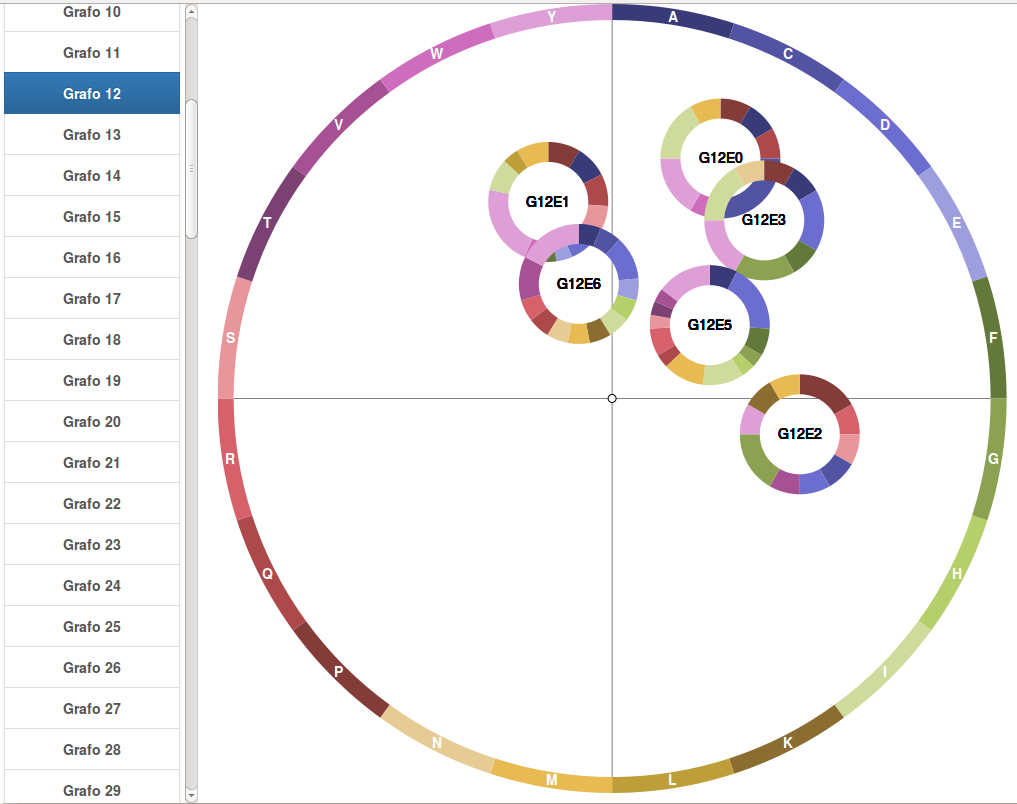
\includegraphics[width=0.8\textwidth]{visualizacao.png}
\end{figure}


\subsection{Posicionamento}
\label{posicionamento}

O posicionamento dos nós na visualização é feito baseado em um sistema de coordenadas polares. A distância de um nó ao centro é inversamente proporcional a similaridade do nó com o centroide computado para todas as pessoas de todos os grafos. Os detalhes do cálculo da similaridade são descritos na Seção~\ref{similaridade}.

O ângulo de um nó é definido primariamente pela categoria de local mais visitada pela pessoa correspondente. Além disso, a segunda categoria mais visitada é usada para gerar uma pequena variação no ângulo, evitando que muitos nós se sobreponham.

Com tal abordagem de posicionamento, procuramos facilitar a comparação entre pessoas da mesma comunidade (grafo) ou de comunidades diferentes. Uma desvantagem observada é que pode haver sobreposições entre elementos semelhantes, tornando a visualização menos legível. A comparação de todos os nós com o centroide foi pensada para que se torne mais fácil identificar as pessoas com hábitos diferentes da média, que estarão mais afastadas do centro.

\subsection{Foco em uma Pessoa}

Embora a exibição inicial use o centroide para computar as similaridades, é possível centralizar a visualização em uma pessoa para melhor analisar a similaridade dela com as demais. Isso acontece ao clicar em um nó. Quanto fazemos isso, a pessoa vai para o centro das coordenadas e todas as outras pessoas ficam posicionadas de acordo com a similaridade entre a pessoa em foco. Podemos inclusive trocar a visualização de grafo que a comparação continuará ativa. Para voltar a comparação com o centroide, basta clicar no pequeno círculo, indicativo da posição do centroide.

\subsection{Cálculo da Similaridade}
\label{similaridade}

Para calcular um índice de similaridade entre as pessoas, adotamos o modelo de espaço vetorial, a métrica TF-IDF ({\em Term Frequency - Inverse Document Frequency}) e a similaridade do cosseno, que são técnicas tradicionalmente utilizados em sistemas de recuperação de informação~\cite{manning2008}. Cada pessoa é representada como um vetor no espaço $n$-vetorial, onde cada dimensão representa uma categoria de local visitado. Seja $p \in P$ uma pessoa do conjunto $P$ de todas as pessoas e $c$ uma categoria de local. Cada componente do vetor é o produto entre os fatores $\text{tf}(c, p) \times \text{idf}(c, P)$, onde:
\begin{itemize}
\item $\text{tf}(c, p)$ é a frequência de visitas de $p$ a locais da categoria $c$.
\item $\text{idf}(c, P)$ é uma medida de quanta informação uma categoria $c$ fornece. Isto é, quanto mais comum é uma pessoa visitar uma categoria, menos representativa ela é para distinguir essa pessoa das demais. O componente $\text{idf}(c, P)$ é computado como:
\begin{align*}
\text{idf}(c, P) = \log \frac{|P|}{1 + |\{p \in P : \text{$p$ visita $c$}  \}|}
\end{align*}
\end{itemize}

Por fim, dados dois vetores $v$ e $u$ de componentes TF-IDF, a similaridade entre eles é calculada usando a similaridade do cosseno, que é definida como:
\begin{align*}
\text{sim}(v, u) = \frac{v \bullet u}{||v|| \times ||u||} = \frac{\sum_{i=1}^{n} v_i \times u_i}{\sqrt{\sum_{i=1}^{n} (v_i)^2} \times \sqrt{\sum_{i=1}^{n} (u_i)^2}}
\end{align*}



\section{Análise dos Dados e Descobertas}

\subsection{Lugares mais visitados}

Foi observado que grande parte dos grafos apresentou uma grande concentração de pessoas no primeiro quadrante (superior direito) da visualização proposta. Isso mostra que as pessoas de tais grafos costumam vizitar mais frequentemente os lugares representados pelo primeiro quadrante. Por outro lado, o terceiro quadrante (inferior esquerdo) apresentou a menor concentração de visitas na grande maioria dos grafos, indicando que as pessoas de tais grafos visitam menos frequentemente, ou não visitam, os lugares representados por tal quadrante. Os quadrantes 2 e 4 apresentaram na maiorias dos grafos a mesma quantidade de visitação aos respectivos lugares, sendo a concentração de pessoas menor que a do primeiro quadrante e maior que a do terceiro quadrante.

\subsection{Costumes similares}

Como discutido na seção anterior, alguns subconjuntos de lugares (quadrantes) apresentam maior ou menor concentração de pessoas. Além disso, foi observado também que o posicionamento dessas pessoas dentro do mesmo quadrante são muito próximos e até mesmo sobrepostos em alguns momentos. Isso mostra que na maioria dos grafos as pessoas possuem costumes similares, no sentido que várias pessoas de um mesmo grafo visitam mais vezes os mesmos lugares.


\footnotesize
\bibliographystyle{abbrv}
\bibliography{tp1}

\end{document}
